\subsection{Road Construction}
This module describes the different road construction algorithms that we tried. As described in the high-level overview of our approach, the best building location is chosen using the getBestMove function and the road is chosen using the findShortestRoad function after the building is chosen. The techniques used in findShortestRoad will be explained in each section.

\subsubsection{Shortest path approach}
The most simple but also efficient way to build roads is choose the shortest road that connects the building to existing roads or edges. The implementation of shortest path is simple. It uses a standard breadth-first search from the building cells to reach the existing roads and edges. This idea also observes the goal to build as few roads as possible, as the road cells generate no score on their own. The shortest path can cause closed vacant areas sometimes, but in most cases, the closed area will be largely filled by future buildings. We also have tried to build roads that cling to existing buildings but this leads to a larger number of unnecessary roads being built. This outweighs the benefits of less white space. This has been confirmed by lower scores in experiments.
% need an image to attest ^ this fact.

\subsubsection{Road pre-building}
The online road-building algorithm can cause problems if large parts of the edge gets covered. This leads to fewer options for new roads being built from the edge. To counter this, we also have tried several pre-building approaches. Before the request comes, we pre-build some roads in a tree-like (fractal) fashion. The idea behind this is to let the road reach larger areas efficiently. But this approach got a lower score than the simple shortest path algorithm. After several experiments, we got the sense that pre-building is not a good idea in this game, as it is very dependent on the distribution and adds more constraints to the later planning.
Figure \ref{fig: prebuildRoad} demonstrate the tree-like pre-build approach.

\begin{figure}
\center
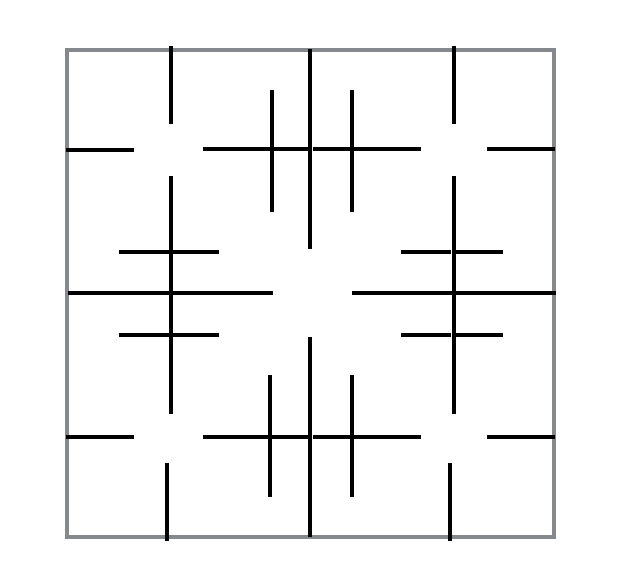
\includegraphics[scale=0.5]{prebuildRoad.png}
\caption{roads grow in fractal manner}
\label{fig: prebuildRoad}
\end{figure}

\subsubsection{close to the buildings}
After dozens of experiments, we finally chose the simple but efficient shortest path strategy. However there may be multiple paths of the same length and we do not arbitrarily pick one like in the previous version. We optimize the simple shortest path strategy by adding a second key which is to measure the perimeter of the road. The perimeter is defined in the same way as the building perimeter we mentioned in the building placement section. Then, our submitted version chooses the road with maximum perimeter among those that have the shortest length. This feature makes a slight difference in the performance, not considerably higher. It does come with the cost of lowering the speed of the algorithm.
